\documentclass{article}
\usepackage{latexsym}
\usepackage{amssymb}
\usepackage{graphicx}
\usepackage{gensymb}
\usepackage[margin=1.2in]{geometry}
\usepackage{float}
\usepackage{wrapfig}
\usepackage{amsthm}
\usepackage{blkarray}
\usepackage{amsmath}
\usepackage{mathtools}
\usepackage{tikz}
\usepackage[]{algorithm2e}
\usepackage{algpseudocode}

\usepackage{framed}
\usepackage{fancyhdr}
\setcounter{page}{0}
\fancypagestyle{plain}{%
\pagestyle{fancy}
\fancyhf{}
\rhead{Tom Goodman}
\lhead{\leftmark}
\chead{Introduction to AI - Exercise I}
\cfoot{\thepage} 
\renewcommand{\footrulewidth}{2pt}}
\pagestyle{plain}
\newcounter{thrmcount}[section]

\usepackage{graphicx}
    \graphicspath{ {/home/txg523/Desktop} }

\newenvironment{thrm}
	{\begin{leftbar}\noindent\ignorespaces\textbf{Theorem \arabic{section}.\arabic{thrmcount}.}\par\noindent\ignorespaces}		
	{\end{leftbar}\stepcounter{thrmcount}\noindent\ignorespaces}
\newenvironment{lem}
	{\begin{leftbar}\noindent\ignorespaces\textbf{Lemma \arabic{section}.\arabic{thrmcount}.}\par\noindent\ignorespaces}		
	{\end{leftbar}\stepcounter{thrmcount}\noindent\ignorespaces}
\newenvironment{nthrm}[1]	
	{\begin{leftbar}\noindent\ignorespaces\textbf{Theorem \arabic{section}.\arabic{thrmcount}.} \textit{(#1)}\par\noindent\ignorespaces}
	{\end{leftbar}\stepcounter{thrmcount}\noindent\ignorespaces}
\newenvironment{nlem}[1]
	{\begin{leftbar}\noindent\ignorespaces\textbf{Lemma \arabic{section}.\arabic{thrmcount}.} \textit{(#1)}\par\noindent\ignorespaces}
	{\end{leftbar}\stepcounter{thrmcount}\noindent\ignorespaces}
\newenvironment{defn}
	{\begin{leftbar}\noindent\ignorespaces\textbf{Definition.}\par\noindent\ignorespaces}
	{\end{leftbar}\noindent\ignorespaces}
\newenvironment{nproof}
	{\begin{proof}}
	{\newline\end{proof}\noindent\ignorespaces}
\newenvironment{prop}
	{\begin{leftbar}\noindent\ignorespaces\textbf{Proposition \arabic{section}.\arabic{thrmcount}.}\par\noindent\ignorespaces}		
	{\end{leftbar}\stepcounter{thrmcount}\noindent\ignorespaces}
\newenvironment{fact}
	{\begin{leftbar}\noindent\ignorespaces\textbf{Fact \arabic{section}.\arabic{thrmcount}.}\par\noindent\ignorespaces}		
	{\end{leftbar}\stepcounter{thrmcount}\noindent\ignorespaces}
\newenvironment{crl}
	{\begin{leftbar}\noindent\ignorespaces\textbf{Corollary \arabic{section}.\arabic{thrmcount}.}\par\noindent\ignorespaces}		
	{\end{leftbar}\stepcounter{thrmcount}\noindent\ignorespaces}	
\newenvironment{ex}[1]
	{\begin{leftbar}\noindent\ignorespaces\textbf{Example.} (\textit{#1})\par\noindent\ignorespaces}
	{\end{leftbar}\noindent\ignorespaces}
\newenvironment{exa}
	{\begin{leftbar}\noindent\ignorespaces\textbf{Example.}\par\noindent\ignorespaces}
	{\end{leftbar}\noindent\ignorespaces}
\newcommand\ddfrac[2]{\frac{\displaystyle #1}{\displaystyle #2}}
\newcommand{\appropto}{\mathrel{\vcenter{
  \offinterlineskip\halign{\hfil$##$\cr
    \propto\cr\noalign{\kern2pt}\sim\cr\noalign{\kern-2pt}}}}}
\title{Goodman's Approximation}
\author{Tom Goodman}
\date{}
\begin{document}
\begin{titlepage}
	\begin{flushleft}
		\vspace*{1cm}
		\Huge
		\textbf{Introduction to AI - Exercise I} \\
		\vspace*{1cm}
		\Large
		\textbf{Tom Goodman} \\
	\end{flushleft}
\end{titlepage}
\newpage
\section{Graph}
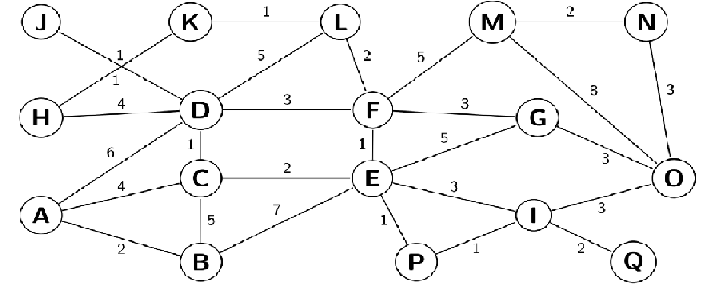
\includegraphics{IntroToAIE1Graph.png}
\section{Question One}
\subsection{Brief}
\textit{For this exercise ignore the path costs. Perform Depth-First-Search to find a path from
A to O. Assume that nodes are expanded in alphabetic order. Write down carefully the
values in your data structures Explored and Frontier as well as the search tree. $[30\% - 30\ marks]$}
\subsection{Answer - Data Structures}
\begin{center}
    \begin{tabular}{ l | c}
    
    \hline
    \textbf{Frontier} & \textbf{Explored}\\
    
    \hline
    $[A_{1}]$ &  [ ] \\ \hline 
    $[B_{2}, C_{3}, D_{4}]$ & $[A_{1}]$ \\ \hline
    $[C_{5}, E_{6}, C_{3}, D_{4}]$ & $[A_{1}, B_{2}]$ \\ \hline    
    $[D_{7}, E_{8}, E_{6}, C_{3}, D_{4}]$ & $[A_{1}, B_{2}, C_{5}]$ \\ \hline
    $[F_{9}, H_{10}, J_{11}, L_{12}, E_{8}, E_{6}, C_{3}, D_{4}]$ & $[A_{1}, B_{2}, C_{5}, D_{7}]$ \\ \hline
    $[E_{13}, G_{14}, L_{15}, M_{16}, H_{10}, J_{11}, L_{12}, E_{8}, E_{6}, C_{3}, D_{4}]$ & $[A_{1}, B_{2}, C_{5}, D_{7}, F_{9}]$ \\ \hline
    $[G_{17}, I_{18}, P_{19}, G_{14}, L_{15}, M_{16}, H_{10}, J_{11}, L_{12}, E_{8}, E_{6}, C_{3}, D_{4}]$ & $[A_{1}, B_{2}, C_{5}, D_{7}, F_{9}, E_{13}]$ \\ \hline
    $[O_{20}, I_{18}, P_{19}, G_{14}, L_{15}, M_{16}, H_{10}, J_{11}, L_{12}, E_{8}, E_{6}, C_{3}, D_{4}]$ & $[A_{1}, B_{2}, C_{5}, D_{7}, F_{9}, E_{13}, G_{17}]$ \\ \hline
        
    \end{tabular}
\end{center}  
\newpage
\subsection{Answer - Tree}    
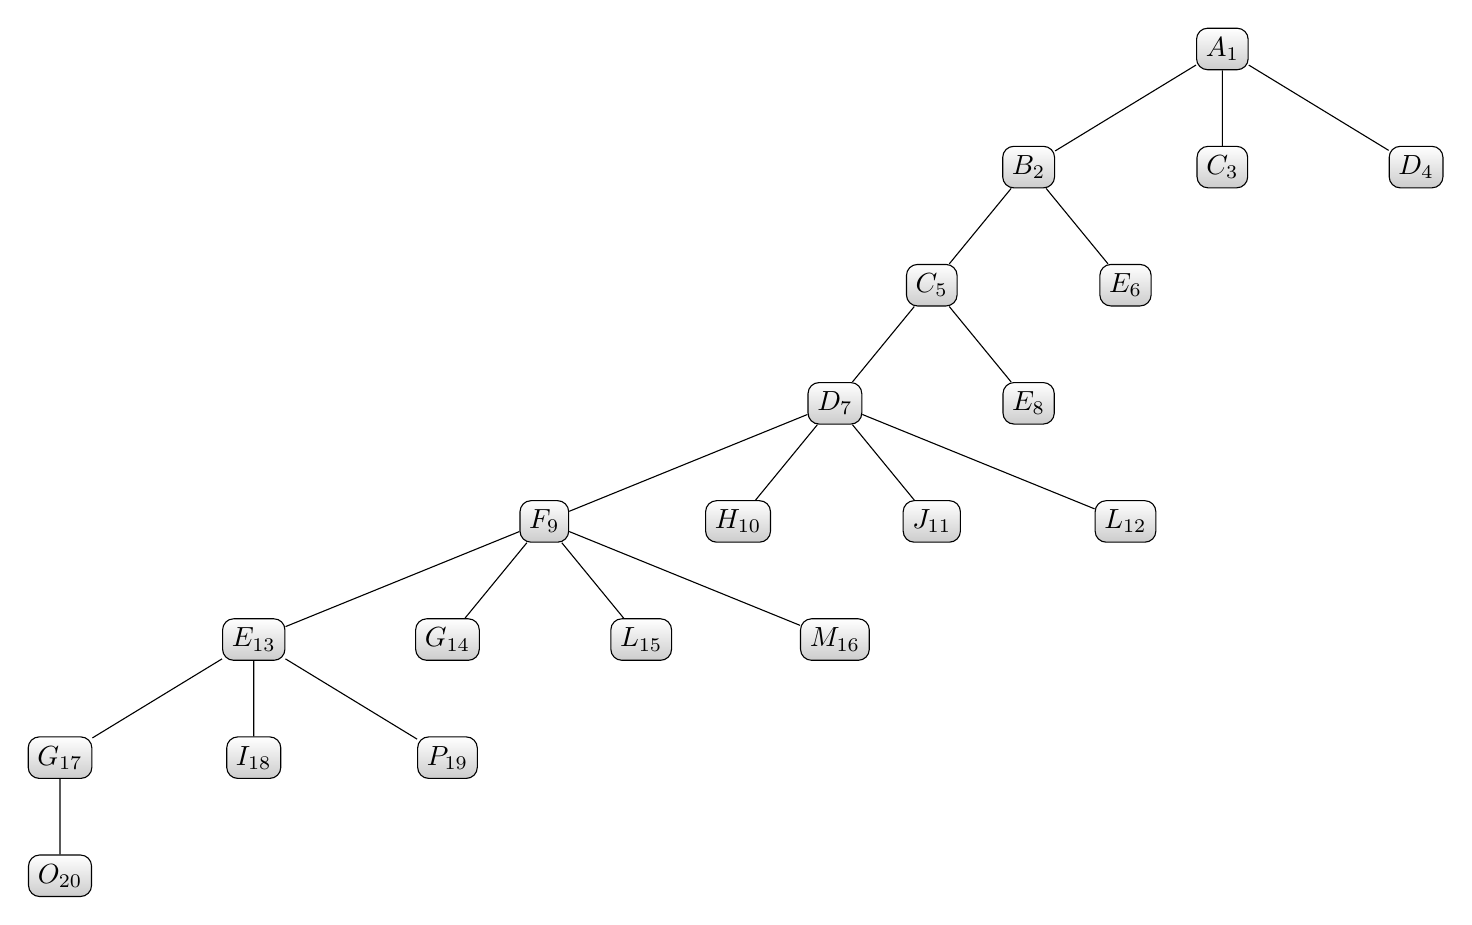
\begin{tikzpicture}[sibling distance=7em, every node/.style = {shape=rectangle, rounded corners, draw, align=center, top color = white, bottom color = black!20}]]
    \node{$A_{1}$}
        child{ node{$B_{2}$}
            child{ node{$C_{5}$}
                child{ node{$D_{7}$}
                    child{ node{$F_{9}$}
                        child{ node{$E_{13}$}
                            child{ node{$G_{17}$}
                                child{ node{$O_{20}$}}}
                            child{ node{$I_{18}$}}
                            child{ node{$P_{19}$}}}                            
                        child{ node{$G_{14}$}}
                        child{ node{$L_{15}$}}
                        child{ node{$M_{16}$}}}
                    child{ node{$H_{10}$}}
                    child{ node{$J_{11}$}}
                    child{ node{$L_{12}$}}}
                child{ node{$E_{8}$}}}
            child{ node{$E_{6}$}}}
        child{ node{$C_{3}$}}
        child{ node{$D_{4}$}};
    \end{tikzpicture} \\
  
\subsection{Answer - Sequence}
The following sequence is the solution to reach the goal state, $\{O\}$.
$$[A_{1}, B_{2}, C_{5}, D_{7}, F_{9}, E_{13}, G_{17}, O_{20}]$$

\newpage
\section{Question Two}
\subsection{Brief}
\flushleft\textit{Perform Uniform Cost Search to find a path from A to O. Again assume that nodes are expanded in alphabetic order. Write down carefully the values in your data structures Explored and Frontier as well as the search tree [30$\%$ - 30 marks]}

\subsection{Answer -Data Structures}
\begin{center}
    \begin{tabular}{ l | c}
    
    \hline
    \textbf{Frontier} & \textbf{Explored}\\
    
    \hline
    [A:0] &  [ ] \\ \hline 
    [B:2, C:4, D:6] & [A:0] \\ \hline
    [C:4, D:6, E:9] & [A:0, B:2] \\ \hline
    [D:5, E:6] & [A:0, B:2, C:4] \\ \hline
    [E:6, J:6, F:8, H:9, L:10] & [A:0, B:2, C:4, D:5] \\ \hline
    [J:6, F:7, P:7, H:9, I:9, L:10, G:11] & [A:0 B:2, C:4, D:5, E:6] \\ \hline
    [F:7, P:7, H:9, I:9, L:10, G:11] & [A:0, B;2, C:4, D:5, E:6, J:6] \\ \hline
    [P:7, H:9, I:9, L:9, G:10, M:12] & [A:0, B;2, C:4, D:5, E:6, J:6, F:7] \\ \hline
    [I:8, H:9, L:9, G:10, M:12] & [A:0, B;2, C:4, D:5, E:6, J:6, F:7, P:7] \\ \hline
    [H:9, L:9, G:10, Q:10, O:11, M:12] & [A:0, B;2, C:4, D:5, E:6, J:6, F:7, P:7, I:8] \\ \hline
    [L:9, G:10, K:10, Q:10, O:11, M:12] & [A:0, B;2, C:4, D:5, E:6, J:6, F:7, P:7, I:8, H:9] \\ \hline
    [G:10, K:10, Q:10, O:11, M:12] & [A:0, B;2, C:4, D:5, E:6, J:6, F:7, P:7, I:8, H:9, L:9] \\ \hline
    [K:10, Q:10, O:11, M:12] & [A:0, B;2, C:4, D:5, E:6, J:6, F:7, P:7, I:8, H:9, L:9, G:10] \\ \hline
    [Q:10, O:11, M:12] & [A:0, B;2, C:4, D:5, E:6, J:6, F:7, P:7, I:8, H:9, L:9, G:10, K:10] \\ \hline
    [O:11, M:12] & [A:0, B;2, C:4, D:5, E:6, J:6, F:7, P:7, I:8, H:9, L:9, G:10, K:10, Q:10] \\ \hline
    [M:12] & [A:0, B;2, C:4, D:5, E:6, J:6, F:7, P:7, I:8, H:9, L:9, G:10, K:10, Q:10, O:11] \\ \hline
        
    \end{tabular}
\end{center}  

\subsection{Answer - Tree}
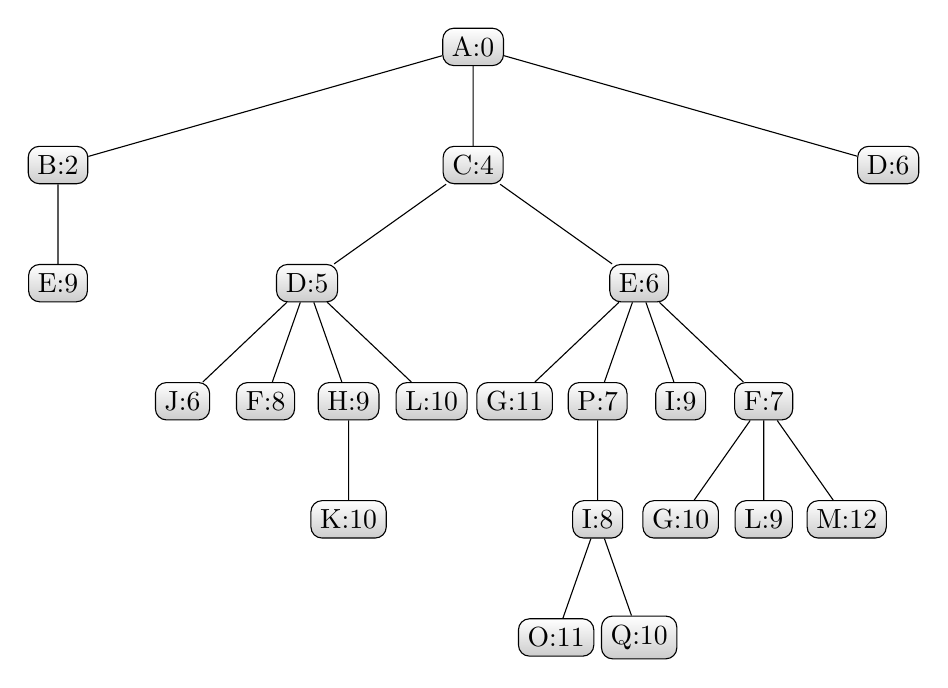
\begin{tikzpicture}[sibling distance=7em, every node/.style = {shape=rectangle, rounded corners, draw, align=center, top color = white, bottom color = black!20}]]
    \node{A:0}[sibling distance=15em]
        child{ node{B:2}
            child{ node{E:9}}}
        child{ node{C:4}[sibling distance = 12em]
            child{ node{D:5}[sibling distance=3em]
                child{ node{J:6}}
                child{ node{F:8}}
                child{ node{H:9}
                    child{ node{K:10}}}
                child{ node{L:10}}}
            child{ node{E:6}[sibling distance=3em]
                child{ node{G:11}}
                child{ node{P:7}
                    child{ node{I:8}
                        child{ node{O:11}}
                        child{ node{Q:10}}}}
               child{ node{I:9}}
               child{ node{F:7}
                   child{ node{G:10}}
                   child{ node{L:9}}
                   child{ node{M:12}}}}}
       child{ node{D:6}};
    \end{tikzpicture} \\
\subsection{Answer - Solution}
The following sequence is the solution to reach the goal state, $\{O\}$.
$$ACEPIO\ (Total\ Cost\ =\ 11)$$
\section{Question 3}
\subsection{Brief}
\flushleft\textit{Ignore again the path costs and perform bi-directional search to solve the problem. [30$\%$ - 30 marks]}
\subsection{Reasoning for the Combination of Searches}
\subsubsection{Breadth-First in both Directions}
Although this method is guaranteed to meet at some point, which will ensure that the search is always complete, the cost of performing the search (memory) is the highest.
\subsubsection{Breadth-First in one direction, Depth-First in the other}
This method is guaranteed to meet, which guarantees completeness. The issue; however, is still the memory usage of a Breadth-First search. As well as this, there is the problem of a difference in memory usage depending on whether the Breadth-First search starts from the start node or the goal node, since the graph is unlikely to be symmetrical.
\subsubsection{Depth-First in both Directions}
This method isn't guaranteed to meet, since the search frontiers of both would be small. Were they to meet;however, the search would almost certainly have a very low time complexity. \footnote{It is worth noting that if the search space was not known to be finite, it would be logical to implement Iterative deepening rather than Depth-First search.}
\\~\\
\textbf{Based on the above information, and the knowledge that the search space is finite, I decided to implement a Depth-first search running in both directions.} 
\subsection{Answer - Data Structures}
Throughout this search, the algorithm checks for a 'meeting point' on generation, not expansion.
\\
\begin{center}
    \begin{tabular}{ l | c}
    
    \hline
    \textbf{Frontier $A$} & \textbf{Explored $A$}\\
    
    \hline
    [$A_{1}$] &  [ ] \\ \hline 
    [$B_{2}, C_{3}, D_{4}$] & [$A_{1}$] \\ \hline
    [$C_{5}, E_{6}, C_{3}, D_{4}$] & [$A_{1}, B_{2}$] \\ \hline
        
    \end{tabular}
    \\~\\
    \begin{tabular}{ l | c}
    
    \hline
    \textbf{Frontier $\Omega$} & \textbf{Explored $\Omega$}\\
    
    \hline
    [$O_{1}$] &  [ ] \\ \hline 
    [$G_{2}, I_{3}, M_{4}, N_{5}$] & [$O_{1}$] \\ \hline
    [$E_{6}, F_{7}, I_{3}, M_{4}, N_{5}$] & [$O_{1}, G_{2}$] \\ \hline
       
    \end{tabular}
\end{center}  
At this point, node E has been generated by both searches. This means that a path to the goal state has been found.
\subsection{Answer - Trees}
\begin{center}
    \begin{tabular}{ l | c}
    
    \hline
    \textbf{Tree $A$} & \textbf{Tree $\Omega$}\\
    
    \hline        
    
    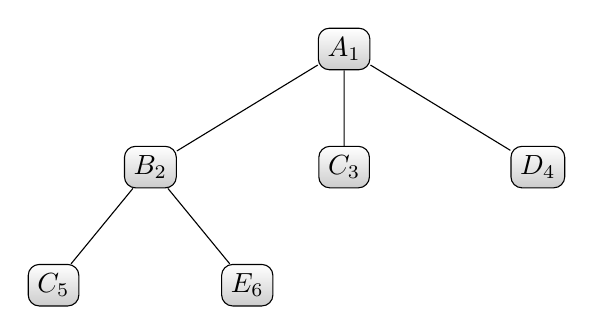
\begin{tikzpicture}[sibling distance=7em, every node/.style = {shape=rectangle, rounded corners, draw, align=center, top color = white, bottom color = black!20}]]
    \node{$A_{1}$}
        child{ node{$B_{2}$}
            child{ node{$C_{5}$}}
            child{ node{$E_{6}$}}}
        child{ node{$C_{3}$}}
        child{ node{$D_{4}$}}; 
    \end{tikzpicture}
        &
     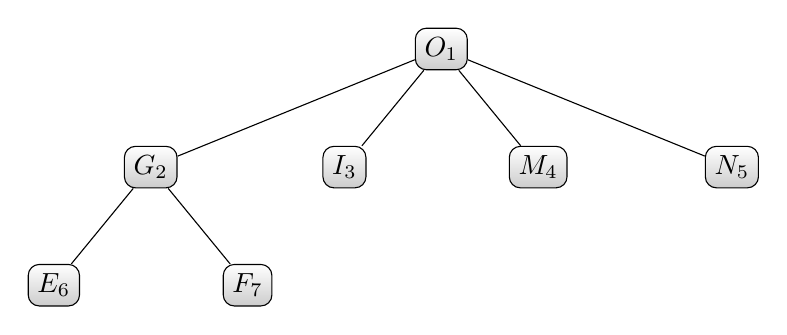
\begin{tikzpicture}[sibling distance=7em, every node/.style = {shape=rectangle, rounded corners, draw, align=center, top color = white, bottom color = black!20}]]
     \node{$O_{1}$}
         child{ node{$G_{2}$}
             child{ node{$E_{6}$}}
             child{ node{$F_{7}$}}}
         child{ node{$I_{3}$}}
         child{ node{$M_{4}$}}
         child{ node{$N_{5}$}};
     \end{tikzpicture}
    
    \end{tabular}
\end{center}    
\subsection{Answer - Solution}
The following sequence is the solution to reach the goal state, $\{O\}$.
$$A,B,E,G,O$$
\newpage
\section{Question 4}
\subsection{Brief}
\flushleft\textit{Design an algorithm for bi-directional search that would allow you to search for an optimal
solution with respect to path costs. [10$\%$ - 10 marks]}
\subsection{Answer}
\textit{let Queue(x, y) $\leftarrow$ Queues node x in queue y} \\
\textit{let Push(x, y) $\leftarrow$ Pushes node x onto stack y} \\
\textit{let Replace(x, y) $\leftarrow$ Replaces node x in priority queue y with the argument x which has a lower total path cost}
\\~\\
$f \leftarrow cumulative\ path\ cost\ from\ the\ start\ state$ \\
$g \leftarrow cumulative\ path\ cost\ from\ the\ goal\ state$
\\~\\
$frontierA \leftarrow prority\ queue\ ordered\ by\ f$ \\
$exploredA \leftarrow queue$ \\
$frontier\Omega \leftarrow priority\ queue\ ordered\ by\ g$ \\
$explored\Omega \leftarrow stack$
\\~\\
\textbf{loop do}\\
\-\hspace{10mm} \textit{//While neither frontier is empty (i.e. while there are still nodes to expand)...}\\
\-\hspace{10mm} \textbf{while} $frontierA\ \neq []\ \&\&\ frontier\Omega\ \neq []$\\
\-\hspace{20mm} \textit{//Checks whether a solution has been found} \\
\-\hspace{20mm} \textbf{for} node in $exploredA$ \\ 
\-\hspace{30mm} \textbf{if} node in $explored\Omega$ \\
\-\hspace{40mm} \textbf{return} solution\ \ \footnote{Dequeues nodes from exploredA and also pops nodes from explored$\Omega$. Also ensures that the common node isn't repeated.} \\ 
\-\hspace{20mm} \textit{//Expands node A} \\
\-\hspace{20mm} $nodeA \leftarrow \ Pop(frontierA)$ \\
\-\hspace{20mm} \textbf{for} childNode attached to nodeA \\
\-\hspace{30mm} \textbf{if} childNode not in $frontierA$ $\& \&$ childNode not in $exploredA$ \\
\-\hspace{40mm} Queue(nodeA, $frontierA$) \\
\-\hspace{30mm} \textbf{else if} childNode in $frontierA$ with higher cost\\
\-\hspace{40mm} Replace(childNode, $frontierA$) \\
\-\hspace{20mm} Queue(node$A$, $exploredA$) \\
\-\hspace{20mm} \textit{//Expands node $\Omega$} \\
\-\hspace{20mm} $node\Omega \leftarrow \ Pop(frontier\Omega)$ \\
\-\hspace{20mm} \textbf{for} childNode attached to node$\Omega$ \\
\-\hspace{30mm} \textbf{if} childNode not in $frontier\Omega$ $\&\&$ childNode not in $explored\Omega$ \\
\-\hspace{40mm} Queue(node$\Omega$, $frontier\Omega$) \\
\-\hspace{30mm} \textbf{else if} childNode in $frontier\Omega$ with higher cost\\
\-\hspace{40mm} Replace(childNode, $frontier\Omega$) \\
\-\hspace{20mm} Push(node$\Omega$, $explored\Omega$) \\
\-\hspace{10mm} \textbf{return} failure \footnote{No path could be found.} \\
\textbf{end}
\\~\\
\newpage
\subsection{Answer - Brief Explanation}
This algorithm works off of the fact that to expand a node, you must have an optimal path to it. If both searches have expanded a node, this means that an optimal path has been found between the start state and the node, and between the node and the goal state. By extension, this means that you have found an optimal path from the start state to the end state.
\\~\\
In order to give a solution, dequeue all of the nodes from $exploredA$ into a set, S, and then pop all of the nodes from $explored\Omega$ into the same set, S. This will give you the solution.
\end{document}